\documentclass{scsSimAUDPaperFormat}
% Beginning of preable.
% Ensure that the copyright notice matches the conference/symposium.
\copyrightnotice{
	SimAUD 2020 May 25-27 Vienna, Austria
	
	\copyright\,2020 Society for Modeling \& Simulation International (SCS)
}
% Load basic packages
\usepackage{balance}		% to better equalize the last page
\usepackage{graphics}		% for EPS, load graphicx instead
\usepackage{times}			% comment if you want LaTeX's default font
\usepackage{url}			% llt: nicely formatted URLs
\usepackage{dblfloatfix}	% allow placement of a page-width figure at top or bottom of page
% llt: Define a global style for URLs, rather that the default one

\usepackage{listings}
\lstdefinestyle{mystyle}{
    %backgroundcolor=\color{backcolour},   
    %commentstyle=\color{codegreen},
    keywordstyle=\color{magenta},
    %numberstyle=\tiny\color{codegray},
    %stringstyle=\color{codepurple},
    basicstyle=\ttfamily\footnotesize,
    breakatwhitespace=false,         
    breaklines=true,                 
    captionpos=b,                    
    keepspaces=true,                 
    numbers=left,                    
    numbersep=5pt,                  
    showspaces=false,                
    showstringspaces=false,
    showtabs=false,                  
    tabsize=2
}
 
\lstset{style=mystyle}

\makeatletter
\def\url@leostyle{%
  \@ifundefined{selectfont}{\def\UrlFont{\sf}}{\def\UrlFont{\small\bf\ttfamily}}}
\makeatother
\urlstyle{leo}

% To make various LaTeX processors do the right thing with page size.
\def\pprw{8.5in}
\def\pprh{11in}
\special{papersize=\pprw,\pprh}
\setlength{\paperwidth}{\pprw}
\setlength{\paperheight}{\pprh}
\setlength{\pdfpagewidth}{\pprw}
\setlength{\pdfpageheight}{\pprh}

% Make sure hyperref comes last of your loaded packages,
% to give it a fighting chance of not being over-written,
% since its job is to redefine many LaTeX commands.
\usepackage[pdftex]{hyperref}
\hypersetup{
pdftitle={SCS Conference Proceedings Format},
pdfauthor={LaTeX},
pdfkeywords={SCS, proceedings, archival format},
bookmarksnumbered,
pdfstartview={FitH},
colorlinks,
citecolor=black,
filecolor=black,
linkcolor=black,
urlcolor=black,
breaklinks=true,
}

% create a shortcut to typeset table headings
\newcommand\tabhead[1]{\small\textbf{#1}}

% create an affilitation superscript
\newcommand{\affiliation}[1]{\ensuremath{^{\textrm{#1}}}}

% End of preamble. Here comes the document.

\begin{document}
\title{
\includegraphics[width=1.0\textwidth]{SimAUDLogo.png}\\\quad\\Modeling and Simulation of Municipal Solid Waste Management System based on Discrete Event System Specification}

% Replace "UniversityA", "CompanyA", "UniversityB" with institution-specific abbreviations.
\def\UniversityA{\affiliation{1}} 
\def\CompanyA{\affiliation{2}}

\author{
	Chang-Hyun Lyoo\UniversityA
	,
	Jinho Jung\UniversityA
	,
	Changbeom Choi\UniversityA
	\,and
	Eun-Young Kim\CompanyA
	\\
	\\
\affaddr{\UniversityA}{Handong Global University, Pohang, Rep. of Korea, \{21300259, 21300704, cbchoi\}@handong.edu}\\
\affaddr{\CompanyA}{Pohang TechnoPark, Pohang, Rep. of Korea, hellosally@daum.net}
}

\maketitle

\begin{abstract}
%생활쓰레기수거는 시민들의 편의에 큰 영향을 미치는 중요한 도시행정서비스이다. 
The cleanliness of the residential area is one of the critical considerations for urban planning.~Especially, municipal waste management is a vital service that raises the resident's satisfaction level.~As the composition of residents in a residential area become complicated, capturing the life patterns of residents is critical for urban planners to achieve the residents' high satisfaction level with the public service.~This paper focuses on representing the temporal behavior pattern of residents in an area as a discrete event system.~Also, this research introduces a simulation environment based on the discrete event system formalism to simulate the life pattern of residents and analyze waste generation and the municipal waste management system.~The simulation results show that modeling the life patterns and the housing types of the residents may represent the dynamics of the waste management system.

\end{abstract}

\keywords{
	Agent-based Simulation; Discrete Event System Formalism; Municipal Solid Waste Management System.
\\
}

% ACM Classification Keywords
\category{I.6.5} \
SIMULATION AND MODELING (Model Development).\\

\section{Introduction}
Today, almost 55\% of the world’s population lives in urban areas, a proportion that is expected to increase to 68\% by 2050~\cite{united20182018}.~Urbanization continues and the population is incessantly increasing.~As the population increases, the total amount of garbage within a local area increases.Among many urban issues, the garbage problem is most closely related to the satisfaction of citizens~\cite{mohit2010assessment}. If garbage is not collected well, it will affect the citizen’s satisfaction and may lead to civil complaints. This will lead to a waste of administrative power and an increase in social costs. Therefore, the urban planners or the employees of the local government should analyze the residential area to estimate the amount of waste generation and provide appropriate public services to the area, such as utilizing garbage trucks to collect wastes.
  
However, it is hard to find models of the residents' life patterns considering the culture and characteristics of residents and the degree of development. The behavior pattern of the residents is more important than the geographic or demographic characteristics of urban areas. In this study, we propose a model focusing on human characteristics and behavior patterns to optimize municipal solid waste management systems. By doing so, we can figure out which waste collection policy would fit and increase the overall satisfaction of citizens.

%DEVS formalism 에 대한 이야기 
Since the behavior of the residents may differ based on their life cycle and occupation, this research utilizes the Discrete Event System Specification(DEVS) formalism to model the behavior of the residents.~The DEVS formalism
is a set-theoretical framework and has a modular characteristic~\cite{Zeigler84, Zeigler90, tms2000}.~As a result, the simulationists may develop their simulation model as a component of the urban system or may reuse a different simulation model which is built by other simulationists.~To maximize the modular characteristic of the DEVS formalism, this research proposes an object-oriented discrete event simulator using the Python programming language.~The simulator captures the default behavior of the residents of the urban area using DEVS formalism and specializes in analyzing the residents by their occupation. Therefore, simulationists may reuse the DEVS simulation model to simulate the temporal behavior of the residents and may differentiate each resident by using occupation objects.

\section{Related Works and Backgrounds}
This section introduces the related works and analyzes them.~Also, it provides the background knowledge to understand the proposed method and the simulation environment.

\subsection{Related Works: Waste Management}
There have been many studies to optimize waste management by applying computer technologies.~Karadmias et al(2006)~\cite{karadimas2006coupling} integrated GIS analysis and agent-based simulation.~Some work has been done to optimize the route of the garbage trucks and reduce waste collection costs using agent-based simulation and Geographic Information System (GIS)~\cite{chalkias2009gis,das2015optimization,nambiar2013multi,nguyenemission,shi2013multi}.
Dao Tuan et al(2017)~\cite{dao2017optimizing} uses ILP and MILP to optimize the route of the garbage trucks considering emission control.~Agent-based simulation and GIS applied waste management system optimizations are proposed in literature~\cite{karadimas2006coupling,shi2013multi,nguyenemission,nambiar2013multi,hua2016towards}.~System dynamics are also used in forecasting the waste generation and simulating an efficient waste management system~\cite{guariso2009modelling,dyson2005forecasting,wang2017system}. Studies regarding optimizing solutions for solid waste management systems are illustrated in Table~\ref{tab:Literatures}.~However, as far as the authors' knowledge, there has been little discussion on the modeling of human behavior patterns or culture.~This study proposes to develop a human-centered model with DEVS formalism. 



\begin{table*}[ht]
\centering
\caption{Area of Interest in the Literatures.}
\begin{tabular}{|c|c|c|c|c|c|c|}
\hline
Authors(year) & GIS & AGENT & DISCRETE & ROUTING & FRAMEWORK & SYSTEM DYNAMICS \\
\hline
Shi, X.et al(2013). & O & O & Hybrid & O & X & X \\
Shi, X.et al(2014) & X & O & Hybrid & X & X & X \\
Guariso, G.et al(2009). & X & X & O & X & X & O \\
Antmann, E.et al(2013). & X & X & O & X & O & X \\
Meng, X. et al(2018). & X & O & X & X & O & X \\
Dyson, B. et al(2005). & X & X & X & X & X & O \\
Wang, C. (2017). & X & X & X & X & X & O \\
Karadimas, N. et al(2006). & O & O & X & X & X & X \\
Nguyen-Trong, K. et al(2017). & O & O & X & O & X & X \\
Nambiar, S. K. et al(2013). & O & O & X & O & X & X \\
Hua, T. M. et al(2016). & O & O & X & O & X & X \\
Das, S. et al(2015). & O & X & X & O & X & X \\
Chalkias, C. et al(2009). & O & X & X & O & X & X \\
Dao-Tuan, A. et al(2017). & O & X & X & O & X & X \\
\hline
\end{tabular}
\label{tab:Literatures}
\end{table*}



%쓰레기 수집 자체 과정에 있어서 쓰레기차의 경로 설정 문제를 다양한 방법들로 해결 한 경우도 있었고,
%쓰레기 수거 및 후처리 시스템 까지 전반적인 시스템을 시뮬레이션한 논문도 있었으나
%특별히 거주민들의 시간적 패턴을 가지고 만족도를 분석한 모델은 존재 하지 않았다.
%그런점에서 우리의 연구는 참신하고 GIS 데이터를 이용하여 단순히 인구를 기준으로 쓰레기의ㅏ 양을 예측하는 %것이 아니라 사람들의 쓰레기 배출 패턴을 시뮬레이션 함으로써 좀더 정확하게 만족도 측정이 가능해졌다.
%다음 연구들의 한계점은 다음과 같다. 
%다른사람이 연구한 방법들에 대해서 소개
%제한점들	ex)문화에 대한 고려가 없었다

\subsection{Backgrounds: Discrete Event System Specification}
The DEVS formalism is a set-theoretic formalism developed for specifying discrete event systems.~The DEVS formalism has two models to represent a discrete event system: the $Atomic~Model$ and the $Coupled~Model$.~The simulationist may specify the behavior of a component of the discrete event system using an atomic model and assembles the Atomic Models to build a bigger system using a Coupled Model.~This research adopts the specification of the Atomic Model to represent the behavior of participant simulation models of urban simulation.~The specification of the Atomic Model is defined as follows.

An Atomic Model is defined as follow:
\begin{tabbing}
xxxx\=xxxx\=xxxx\=xxxx\=\kill\\
\> \> \> $AM$ = $<X, Y, S, \delta_{ext}, \delta_{int}, \lambda, ta>$\\
where\\
\> $X$: a set of external input event types,\\
\> $Y$: an output set,\\
\> $S$: a sequential state set,\\
\> $\delta_{ext}$: $Q \times X \rightarrow S$, an external transition function\\
\> \> where $Q$ is the total state set of \\
\> \> $M$ = $\{(s,e)|s \in S\:and\:0 \leq e \leq ta(s)\}$,\\
\> $\delta_{int}$: $S \rightarrow S$, an internal transition function,\\
\> $\lambda$: $S \rightarrow Y$, an output function,\\
\> $ta$: $S \rightarrow {\cal R}^{+}_{0,\infty}$, a time advance function, \\
\> \> where ${\cal R}^{+}_{0,\infty}$ is the non-negative real numbers \\
\> \> with $\infty$ adjoined.
\end{tabbing}

An atomic model $AM$ is a model which is affected by external input events
$X$ which in turn generates output events $Y$.~The state set $S$ represents the unique description of the model.~The internal transition function $\delta_{int}$ and the external transition
function $\delta_{ext}$ compute the next state of the model.
If an external event arrives at the elapsed time $e$ which is less than or
equal to $ta(s)$ specified by the time advance function $ta$, a new
state $s'$ is computed by the external transition function $\delta_{ext}$.~Then, a new $ta(s')$ is computed, and the elapsed time $e$ is set to zero.
Otherwise, an internal event arrives at $ta(s)$, and then a new state
$s'$ is computed by the internal transition function $\delta_{int}$.
In the case of internal events, the output specified by the output function
$\lambda$ is produced based on the state $s$, which means the output function
is processed before the internal transition function.
Then, as before, a new $ta(s')$ is computed, and the elapsed time $e$ is set to zero. 

\begin{figure}[!h]
    \centering
    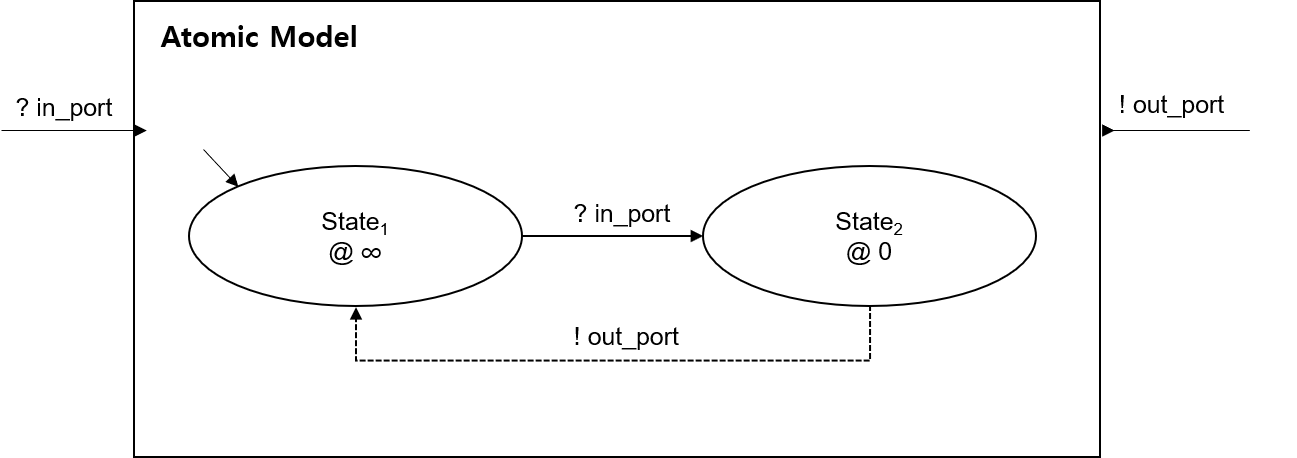
\includegraphics[width=1.0\columnwidth]{fig/Atomic_model}
    \caption{Example of an Atomic Model}
    \label{Fig:AtomicModel}
\end{figure}

Figure~\ref{Fig:AtomicModel} shows the diagram of an Atomic Model.~The label starting with the question mark denotes the input port, and the label starting with the exclamation mark denotes the output port.~The ellipse shows the state of the model and ellipse with an arrow denotes the initial state of the model.~Each state has the state name and the positive real number which denotes the occupancy time.~When the elapsed time meets the occupancy time, the simulation algorithm will trigger the output function and internal transition function, sequentially. 

The proposed simulator partially accepts the notation of DEVS formalism and its simulation algorithm.~Listing~\ref{lst:atomic} shows the python code of the example atomic model.~As shown in the Listing~\ref{lst:atomic}, the proposed simulator provides a programming interface that has a one-to-one correspondence with the Atomic Model specification of the DEVS formalism.


\begin{lstlisting}[language=Python, caption=Example Code of Atomic Model, label={lst:atomic}]
class AtomicModel(BehaviorModelExecutor):
    def __init__(self, instance_time, destruct_time, name, engine_name):
        BehaviorModelExecutor.__init__(self, instance_time, destruct_time, name, engine_name)

        self.init_state("State1")
        self.insert_state("State1", Infinite)
        self.insert_state("State2", 0)

        self.insert_input_port("in_port")
        self.insert_output_port("out_port")

    def ext_trans(self,port, msg):
        if port == "in_port":
            self._cur_state = "State2"

    def output(self):
        name = self.get_name()
        msg = SysMessage(name, "out_port")
        return msg
        
    def int_trans(self):
        if self._cur_state == "State2":
            self._cur_state = "State1"
\end{lstlisting}

\section{Proposed Method and Environments}

This section introduces the proposed method to model the municipal solid waste management system and its simulation environment.~To capture the dynamic behavior of the residents, we classified the type of residents and modeled them in the object-oriented fashion.~After modeling the residents, we developed a simulation model to represent the housing types. ~Finally, we developed simulation models to provide municipal solid waste management services to the residents. 

To model the residential area,~\begin{figure}[!ht]
    \centering
    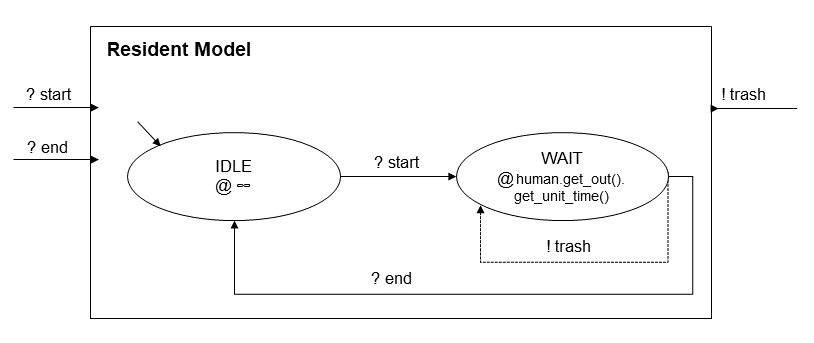
\includegraphics[width=1.0\columnwidth]{fig/resident_model.jpg}
    \caption{Atomic Model of a Resident}
    \label{Fig:residentmodel}
\end{figure}
Figure~\ref{Fig:residentmodel} shows the diagram of a Resident Model.~It describes the life patterns of residents, such as wake up, sleep, in, $Leave\ time$, $Amount\ of\ Waste\ Emission$ differently from each job. Based on the survey of "What time did you wake up today?" conducted by Gallup Korea in 2013, we divided jobs into seven types [(Agriculture, Forestry and Fisheries(AFF)), Student, Housewife, Construction Worker, White collar, Inoccupation and Self-employment] and set different life patterns for different types of people~\cite{gallup2013}.~Set the $Leave\ time$ differently each time using a normal distribution for the given average $Leave\ time$.~Each $Leave\ time$, residents send $Amount\ of\ Waste\ Emission$ to their family model and check model.
\begin{figure}[!ht]
    \centering
    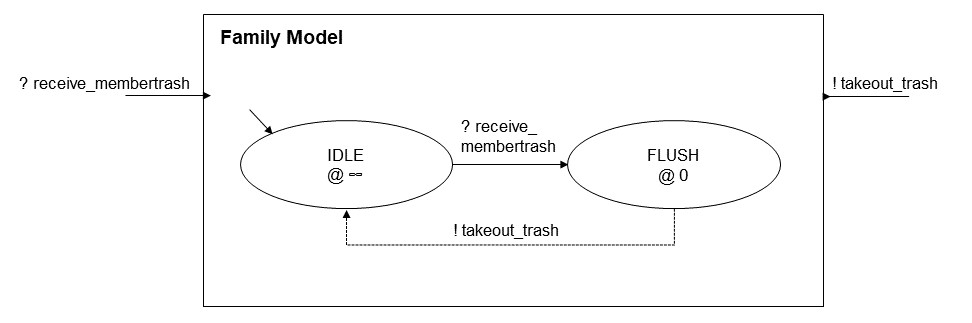
\includegraphics[width=1.0\columnwidth]{fig/family_model.jpg}
    \caption{Atomic Model of a Housing Type}
    \label{Fig:Familymodel}
\end{figure}
Figure~\ref{Fig:Familymodel} shows the diagram of a Family Model.~Family models are a set of resident models. We created a family model to implement the actual furniture and randomly linked residents to the family model.~Depending on the number of families, each family's garbage storage size and the $Leave\ time$ will vary.~Receive garbage data from the resident model through the receive-membertrash port and add it to the current storage size.~If the current storage size is larger than the garbage storage size, one random member of the family was selected to take out trash based on the $Leave\ time$ of the selected person.~Transfer current storage size to the garbage can model through the takeout-trash port and change the current storage size to 0.
\begin{figure}[!ht]
    \centering
    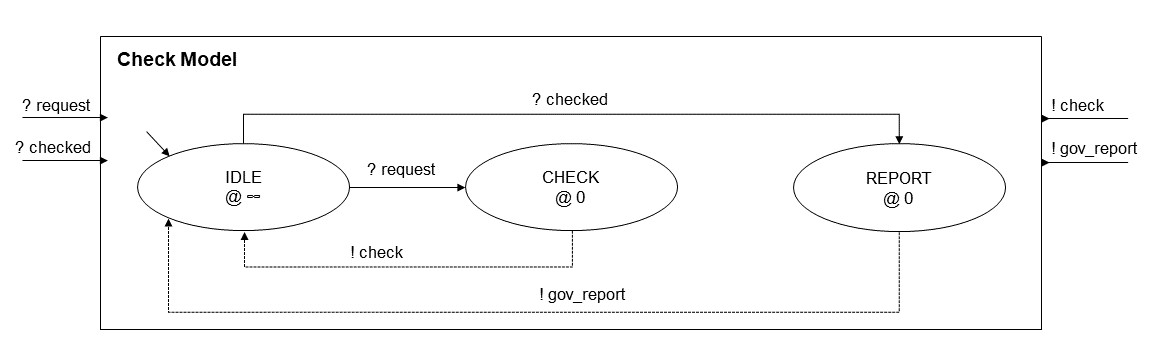
\includegraphics[width=1.0\columnwidth]{fig/check_model.jpg}
    \caption{Atomic Model to Check the garbage}
    \label{Fig:Checkmodel}
\end{figure}
Figure~\ref{Fig:Checkmodel} shows the diagram of a Check Model.~This is the measurement model for the residents' satisfaction according to the capacity of the garbage can.~The residents' satisfaction with the cleanliness of the garbage collection site is measured every $Leave\ time$.~When the Check Model receives a request message from the Resident model, a check message is sent to the garbage can model to check the status of the garbage can.If the value of the garbage can ratio from the garbage can model was received through the check port, the satisfaction level of the individual was measured with the garbage can ratio.~If the satisfaction level falls below a certain number, a message is sent to the Government Model through the gov-report port.
\begin{figure}[!ht]
    \centering
    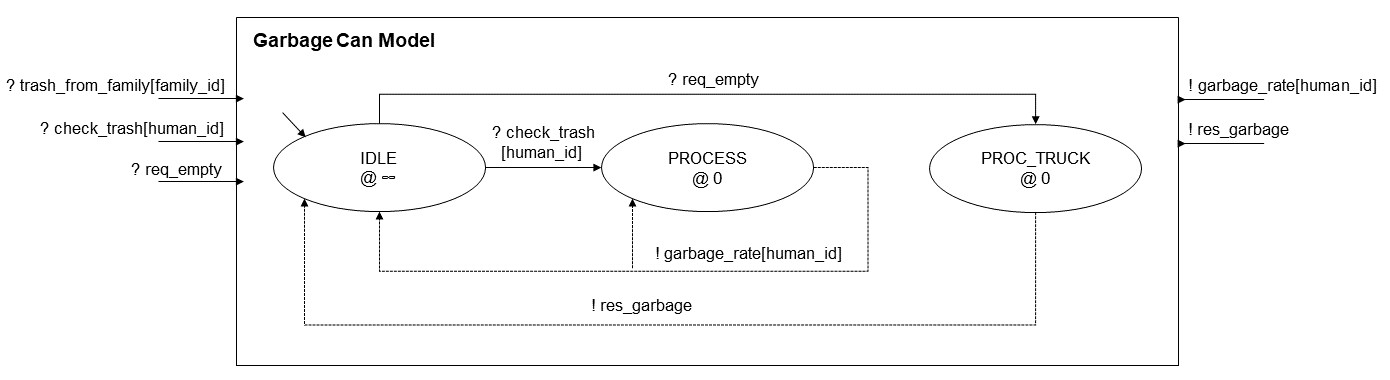
\includegraphics[width=1.0\columnwidth]{fig/garbagecan_model.jpg}
    \caption{Atomic Model to Calculate the garbage of a Building}
    \label{Fig:Garbagemodel}
\end{figure}
Figure~\ref{Fig:Garbagemodel} shows the diagram of a Garbage Model.~It is a model that measures the waste taken out from each building.~By setting the size of the garbage can at random, we can observe changes in the residents' satisfaction according to the capacity of the garbage can.~This allows you to measure the capacity of the proper garbage's size according to the residents.The value of the garbage can was added by receiving the value of takeout-trash from the Family Model.~When prompted to check the status of the garbage in the Check Model, the ratio of the garbage was calculated and sent to the Check Model.~When you receive an empty message from the Garbagetruck Model, the accumulated amount of Garbage is sent to the Garbagetruck Model.
\begin{figure}[!ht]
    \centering
    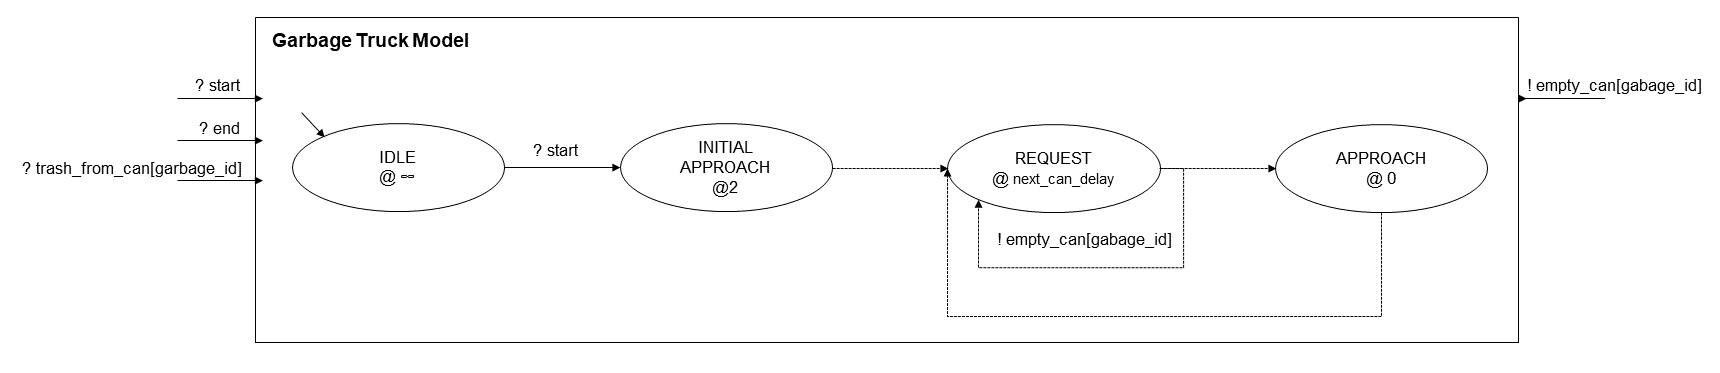
\includegraphics[width=1.0\columnwidth]{fig/garbagetruck_model.jpg}
    \caption{Atomic Model to Collect the garbage in a building}
    \label{Fig:garbageTruckmodel}
\end{figure}
Figure~\ref{Fig:garbageTruckmodel} shows the diagram of a Garbagetruck Model.~This model is designed to retrieve garbage from buildings in a fixed area at regular intervals.~The order of the buildings, the collection time for each building, the capacity of the garbage truck, and the collection cycle can be determined by parameters.~Each parameter can be adjusted to create an optimized resource circulation system for each region. The trash data from Garbage can is optained in the prescribed order and added to the truck-current-storage.~Then it sends a message that makes the capacity of the Garbage can zero.~This is repeated until all schedules are run, and when all schedules are finished, the truck-current-storage is initialized to zero and the schedule is repeated according to the collection cycle.
\begin{figure}[!ht]
    \centering
    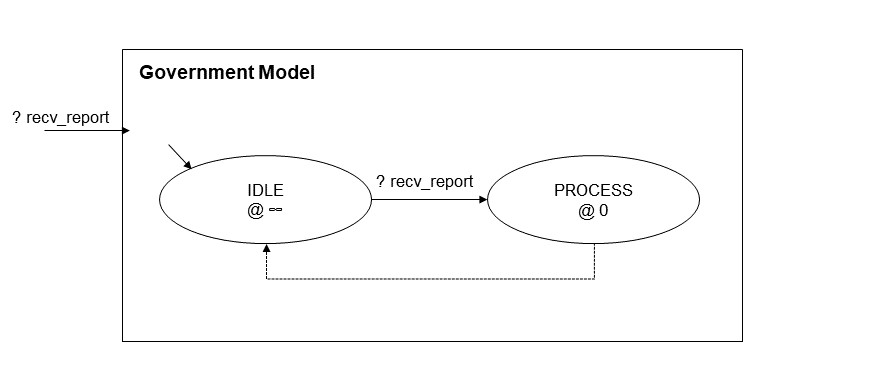
\includegraphics[width=1.0\columnwidth]{fig/government_model.jpg}
    \caption{Atomic Model to Receive report from Resident}
    \label{Fig:Governmentmodel}
\end{figure}
Figure~\ref{Fig:Governmentmodel} shows the diagram of a Government Model.~This model is designed to reduce complaints and improve satisfaction by changing the operation time or the number of operations of the garbage truck according to the residents' complaints.~The current model only receives the message when the report message from the Check Model and does not do anything else.
% 모델링을 어떻게 했다. 
% 사람, 직업, 행위에 대해서 모델링을 어떻게 했다고 작성

%우리가 하려는 것들
%Behaviourmodel, Familymodel, garbagecan, garbagetruck, checker 등등 
%상속 하는 그림,
%각 모델에서 설명 (human - 직업)
%직업이 simulation에 영향을 줌 -> 직업별 행동패턴을 부여해서 모델링 하는게 좋다
%Report하는 사람과 안하는 사람 리스트나 튜플 형태로 표현


\begin{figure*}[ht]
    \centering
    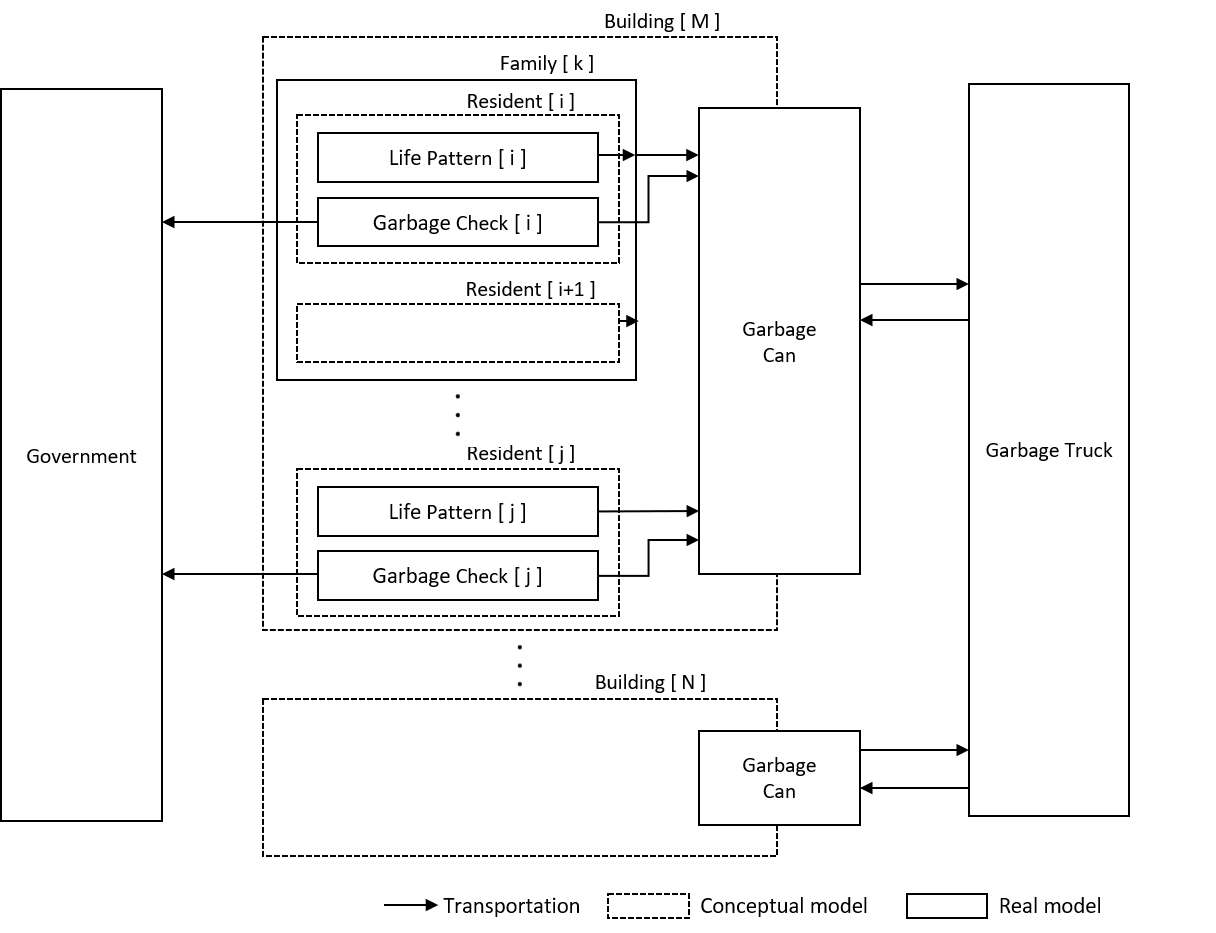
\includegraphics[width=1.5\columnwidth]{fig/Framework}
    \caption{Atomic Model to Calculate the Satisfaction Level of a Resident}
    \label{Fig:Framework}
\end{figure*}


Figure~\ref{Fig:Framework} shows the overall framework of the proposed simulation environment.~The urban planner may compose the simulation models to represent the residential areas by connecting the ports to the other simulation models' port.

\section{Case Study}

\장량동 다 날려야함 ㅠㅠ

This section illustrates the case study of the proposed method and the simulation environments.~This research models the Jang-Ryang district of the Pohang city in the Republic of Korea.~The composition of the residents in Jang-Ryang district is different from other residential areas.~There are two colleges and one university located nearby, so many students live in a studio apartment complex during the academic year.~Also, the portion of the construction workers grows and subsides due to the construction plan of the city.~The behaviors of the college students and the construction workers are different. 
\begin{figure}[!ht]
    \centering
    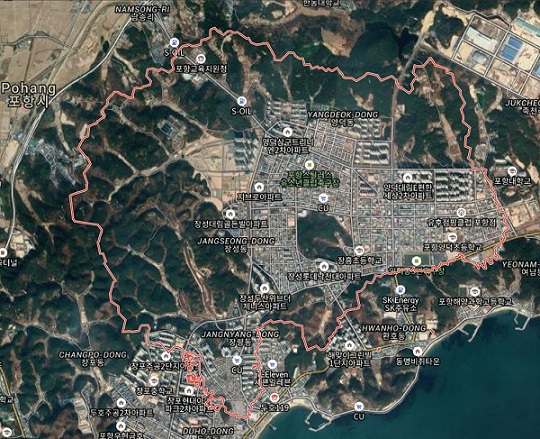
\includegraphics[width=1.0\columnwidth]{fig/map.jpg}
    \caption{Map of Jangryang-dong, Pohang represented within the red bold lines}
    \label{Fig:JangYrang}
\end{figure}
\subsection{Assumptions and the Simulation Parameters}
The following are assumptions made for modeling the  Jang-Ryang destrict
\begin{itemize}
    \item Each building has a garbage can to hold the garbage temporarily.
    \item Each resident has their own schedule to go out.
    \item Every resident takes out garbage every day when they go out. 
    \item If residents have a family, they take out garbage as a family together.
    \item The garbage truck collects the garbage from the building regularly.
    \item The satisfaction level of the resident may change at the moment when resident take out the garbage.
    \item The resident may complain to the Government when the garbage goes above a certain level.
\end{itemize}



%As of February 2019, 71,802 people are currently residing in this area.
%Pohang city, the Republic of Korea began to develop after Pohang Iron and Steel Company was established in 1968. Jangryang district was only a remote village with a population of more than 1,900 in 1981. In the early 2000s, many apartments were built and a bed town was formed under the city development plan. The population began to move in as long-range housing districts were formed. The largest population in Pohang has been living in Jangryang-dong since 2011. As of February 2019, 71,802 people are currently residing in this area. The ratio of blue collars is high as the industrial complex's full-fledged operation brings in the population. Since convenient traffic conditions and commercial districts are easy to bring in tenants, most of the real-life residents are short-term residents. Also, there are two colleges and one university located nearby, so many students live in a studio apartment complex during the school year. 

%The prediction of municipal solid waste generation plays an important role in a solid waste management.

\begin{table*}[ht]
\centering
\caption{Description of Simulation Parameters}
\begin{tabular}{|l|c|c|}
\hline
 & Construction Worker & Student \\ \hline
Leave Time & 6:22:00 & 7:58:00 \\ \hline
Amount of Waste Emission & 0.9 & 0.9 \\ \hline
Satisfaction Function & 
    $Satis(x) = \begin{cases}
              + 10 & \text{if } x < 0.8,\\
              \ \ \ 20 & \text{if } x = 0,\\
               -10 & \text{if } x > 0.8
          \end{cases}$
 & $Satis(x) = \begin{cases}
              + 10 & \text{if } x < 0.8,\\
              \ \ \ 20 & \text{if } x = 0,\\
               -10 & \text{if } x > 0.8
          \end{cases}$ \\ \hline
\end{tabular}
\label{tab:SimParam}
\end{table*}
Following Table~\ref{tab:SimParam} shows the simulation parameters deduced from the assumptions.~$Leave\ Time$ represents an interval at which one leaves one's home.~We modified the $Leave\ time$ based on average wake-up time data from living time survey~\cite{gallup2013}.~$Amount\ of\ Waste\ Emission$ represents the amount of waste generated until out time. For realistic simulation, The amount of waste generation of the residents is drawn from average waste emissions per capita~\cite{Korea_resource_recirculation_information_system_2018}.~$Satisfaction\ Function$ represents one's satisfaction level according to the level of garbage. Based on the experiences of some students, the decision made by the heuristic.

% 이상의 파라미터 값이 어떻게 책정되었는지가 설명되어야 함


%\\
\subsection{Jang-Ryang District Model and Simulation Results}

The experiment was conducted using the above simulation environment on AWS C9 IDE.~The experiment was conducted in three different combinations;only students; only construction workers; and student and construction Workers.~Each case was run 30 times with different random number sequences.~The first case reported the highest number of complaints(only students) and the results varied depending on the proportion of the residents.~According to the satisfaction function used above, if the resident's satisfaction falls once and the complaint is raised, then one's satisfaction level rarely becomes normal.~In other words, when a resident raises complaint once, then one continues to file a complaint with a high probability.
%한번 만족도가 내려가면 잘 올라오지 않고, 계속해서 report를 한다. 

Figure ~\ref{Fig:case_result} shows average number of reports. Average number of reports differ from each composition of the ratio of residents.
\begin{figure}[!h]
    \centering
    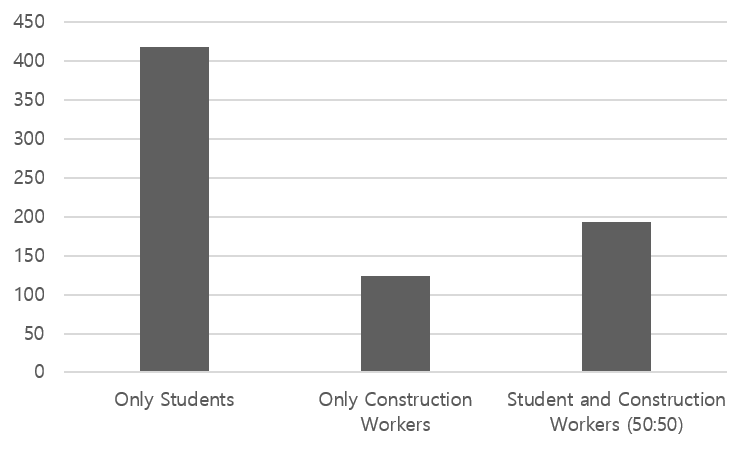
\includegraphics[width=1.0\columnwidth]{fig/case_study_result.png}
    \caption{Number of complaints filed according to the ratio of resident occupations}
    \label{Fig:case_result}
\end{figure}

\section{Conclusion}
%우리의 모델은 훌륭했다. 하지만 UI 적으로 공무원들이나 일반인들이 사용하기에는 무리가 있을것으로 예상된다. 이 부분을 보완해서 나중에 FLASK등과 연결하여 쉬운 인터페이스로 작동하도록 하면 좋을 것 같다.
As the complexity of an urban area increases, estimating waste generation and providing an alternative solution for waste collection are important for urban planners and employees of the local government to increase the satisfaction level of residents.To compute the approximated satisfaction level of residents, this research modeled the residents' life patterns and housing types to estimate waste generation and collection.~This research models the behavior of the resident, housing type and waste management system as a discrete event system.~To model and simulate the system, this research adopts the DEVS formalism and implement the simulation algorithm to analyze an urban area. 

For the future research guideline, attaching GIS to reflect the real-world data or implementing a graphical user interface to increase the usability to urban planners or the employees of the local government can be considered.



\balance

\bibliographystyle{unsrt}
\bibliography{References}

\end{document}
